\documentclass{report}
\usepackage[utf8]{inputenc}
\usepackage{amsmath, amsfonts, amsthm, graphicx, geometry, lipsum}
\usepackage{natbib}
\usepackage[spanish]{babel}
\usepackage{hyperref}
\hypersetup{
    colorlinks=true,
    linkcolor=blue,
    urlcolor=red,
    pdftitle={Tarea 4: Optimización en redes},
    }
\usepackage{fancyvrb}
\usepackage{fancyhdr, lastpage}
\pagestyle{fancy}
\lhead{Optimización en Redes}
\rhead{Universidad Autónoma de Nuevo León}
\cfoot{Page \thepage\ of \pageref{LastPage}}

\usepackage{etoolbox} %Use carefully!
\patchcmd{\chapter}{\thispagestyle{plain}}{\thispagestyle{fancy}}{}{}

\usepackage[Glenn]{fncychap}
%Options: Sonny, Lenny, Glenn, Conny, Rejne, Bjarne, Bjornstrup

\usepackage{xcolor}
\usepackage{tikz}
\usepackage[most]{tcolorbox}

\newtcbtheorem{theo}%
  {Theorem}{}{theorem}
  
\usepackage{siunitx}
\usepackage{setspace}
\onehalfspacing

%#TODO comandos nuevos
\newcommand{\dij}{{\bfseries {\textit{Dijkstra }}}}
\newcommand{\bell}{{\bfseries {\textit{Bellman Ford }}}}

\begin{document}

\tableofcontents
\newpage
\section{Algoritmo \dij}
Para el algoritmo de \dij hay dos archivos en el cual podemos resolver un grafo, ya sea directo o sin dirección. El primero con el nombre de shortest\_path2.py se utiliza una función con el nombre \dij, el cual toma el grafo en términos de diccionario, el nodo de inicio, el nodo destino, las etiquedas debidamente inicializadas en $\infty$ y la dimensión de este mismo grafo definido.

En el mismo código se da la opción de escoger entre tres grafos de los cuales ningún costo es negativo, puesto que \dij solo trabaja con costos positivos.

En el primer ejemplo tenemos el siguiente grafo:
\begin{figure}[ht]
    \centering
    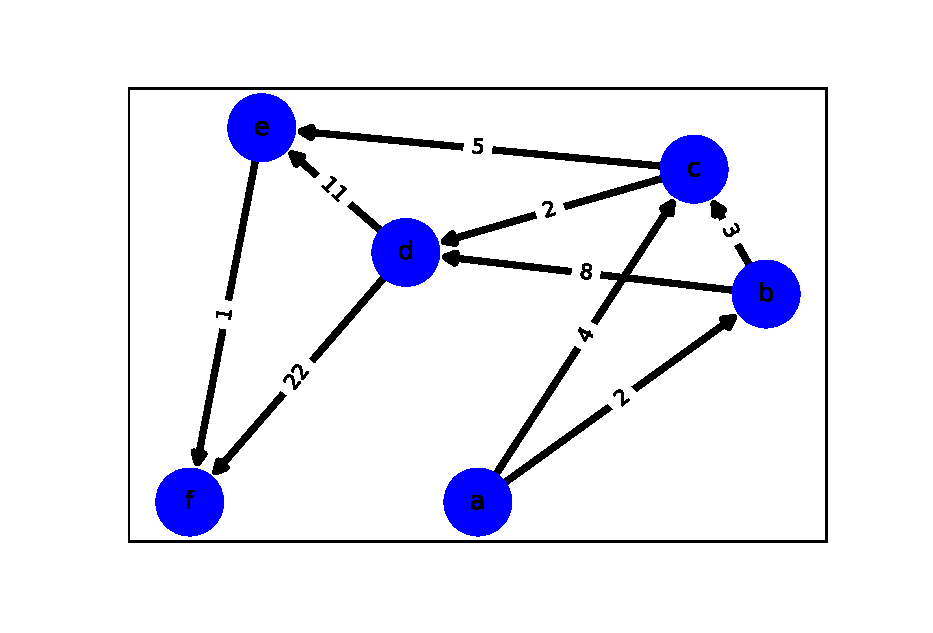
\includegraphics[scale = 0.4]{ejemplo1.eps}
    \label{figura1}
    \caption{6 nodos, inicio = a, final = f}
\end{figure}

Como se muestra en la figura 1,tenemos un grafo de 6 nodos, comenzamos en el nodo a y terminaremos en el nodo f, después de aplicar el algoritmo \dij encontramos como solución:
\begin{center}
    Distancia más corta:
    10,
    ruta de la distancia más corta:
    ['a', 'c', 'e', 'f']
\end{center}

Para el ejemplo 2 tenemos el siguiente grafo:

\begin{figure}[h!t]
    \centering
    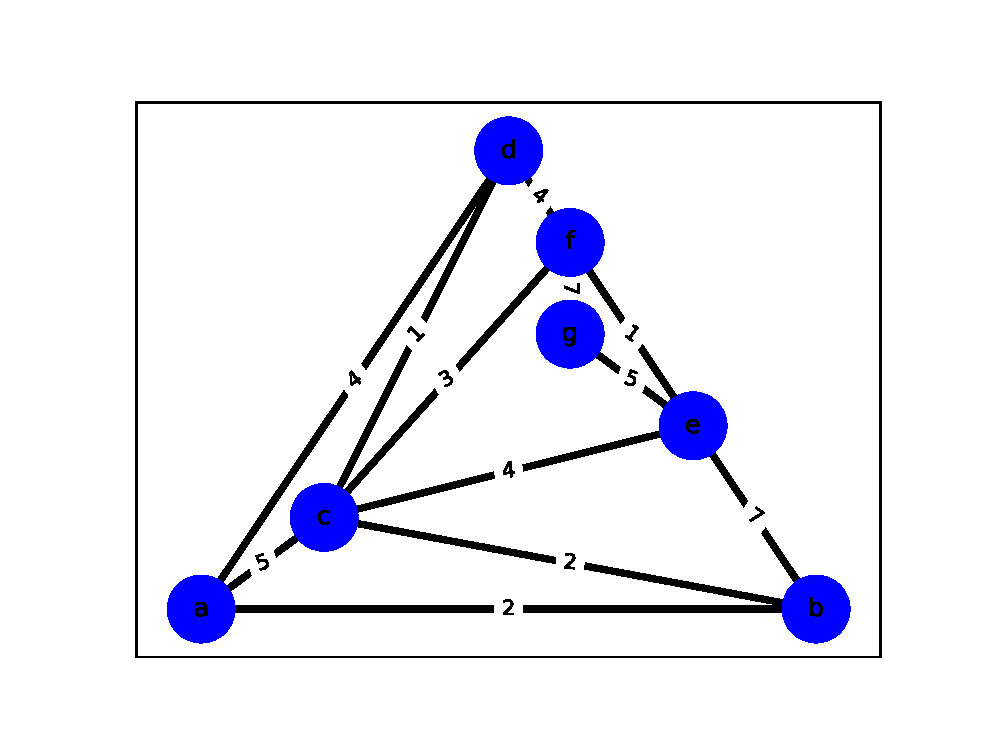
\includegraphics[scale = 0.35]{ejemplo2.eps}
    \label{figura2}
    \caption{7 nodos, inicio = a, final = g}
\end{figure}

Como vemos en el título de la  figura 2,tenemos un grafo de 7 nodos, comenzamos en el nodo a y terminaremos en el nodo g, después de aplicar el algoritmo  \dij nos encontramos con la solución:
\begin{center}
    Distancia más corta:
    13,
    ruta de la distancia más corta:
    ['a', 'b', 'c', 'e', 'g']
\end{center}

En el último ejemplo, tenmos el siguiente grafo:

\begin{figure}[h!t]
    \centering
    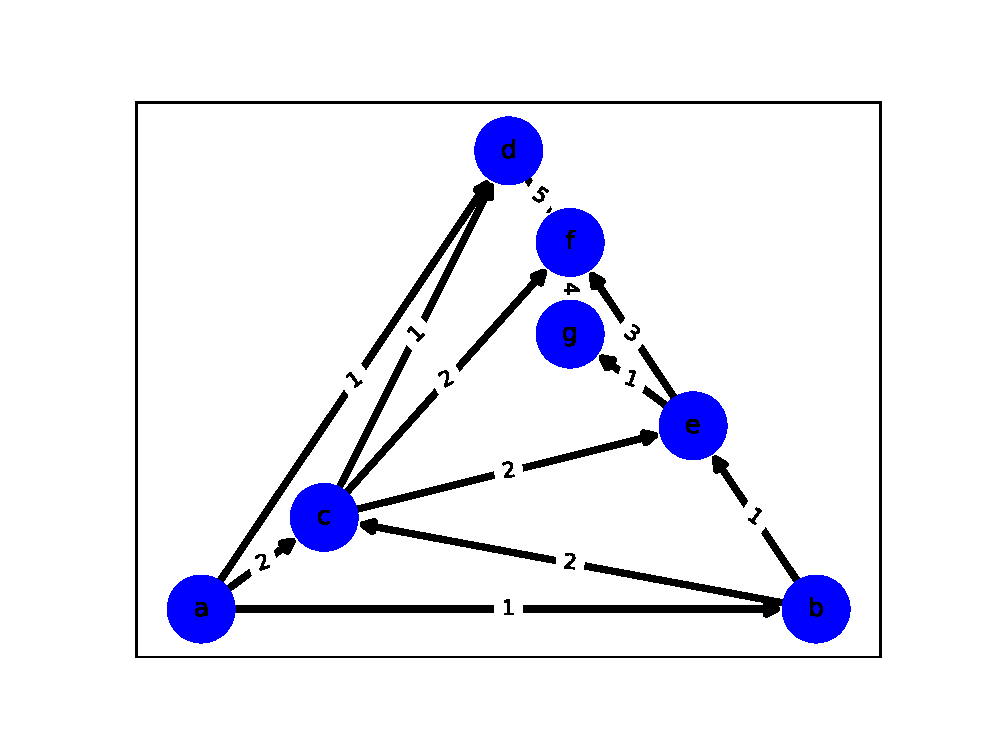
\includegraphics[scale = 0.4]{ejemplo3.eps}
    \label{figura3}
    \caption{7 nodos, inicio = a, final = g}
\end{figure}

Como vemos en el título de la  figura 3, tenemos un grafo de 7 nodos, comenzamos en el nodo a y terminaremos en el nodo g, después de aplicar el algoritmo  \dij nos encontramos con la solución:
\begin{center}
    Distancia más corta:
    3,
    ruta de la distancia más corta:
    ['a', 'b', 'e', 'g']
\end{center}

\section{Algoritmo \bell}

En el algoritmo de \bell se procedió de manera similar al algoritmo \dij nos encontramos con la distancia más corta pero tomando distancias negativas.

Para este algoritmo se corrieron los mismo tres grafos anteriores obteniendo los mismos resultados, además se agregaron unos ejemplos más pero con costos negativos, que veremos a continuación.

Para el ejemplo 1 con costos negativos tendremos el siguiente grafo:
\newpage

\begin{figure}[h!t]
    \centering
    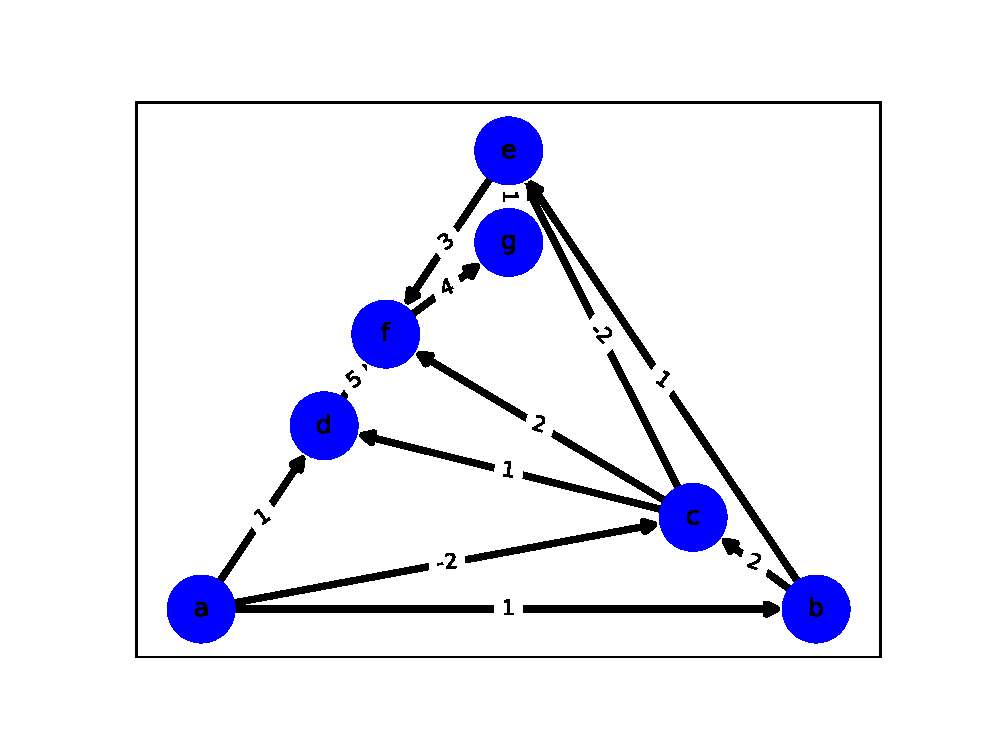
\includegraphics[scale = 0.5]{ejemplo4.eps}
    \label{figura4}
    \caption{6 nodos, inicio = a, final = f}
\end{figure}

El cual es un grafo no dirigido de 6 nodos con dos costos negativos, al aplicar el algoritmo \bell obtenemos que el grafo tiene un ciclo negativo.

En el ejemplo 2 tenemos también un grafo no dirigido que es el siguiente:

\begin{figure}[h!t]
    \centering
    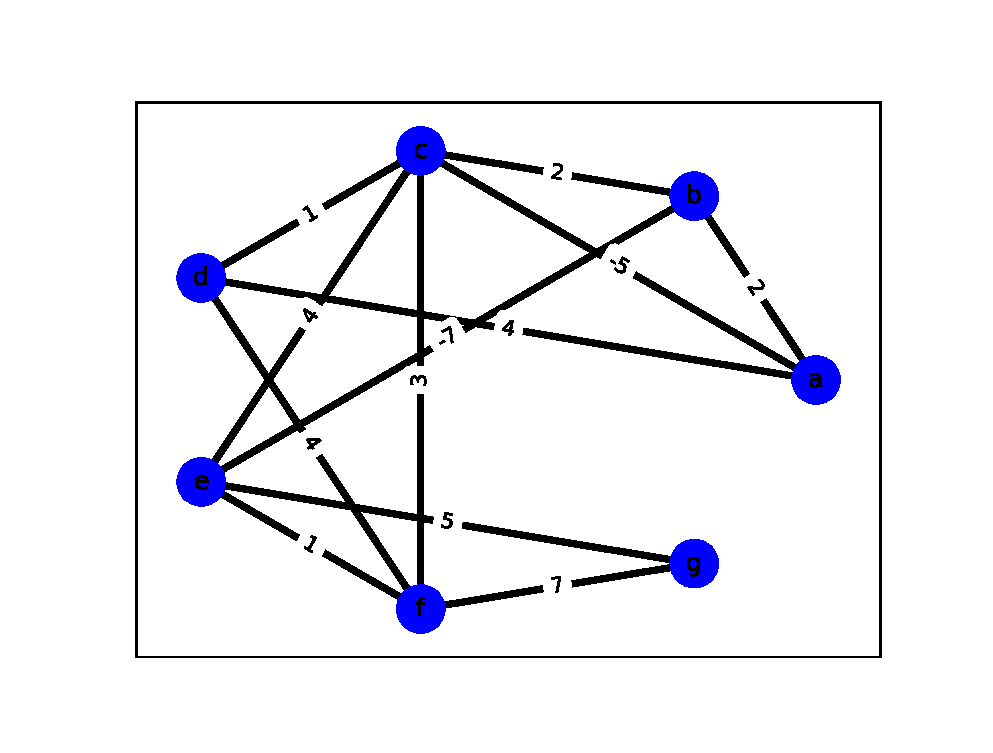
\includegraphics[scale = 0.5]{ejemplo5.eps}
    \label{figura5}
    \caption{7 nodos, inicio = a, final = g}
\end{figure}

De igual manera que el anterior tenemos un grafo no dirigido pero ahora de 7 nodos el cual tiene de igual manera dos valores negativos, y otra vez al aplicar el algoritmo \bell obtenemos que tiene un ciclo negativo.

En el ejemplo 3, tenemos un grafo dirigido el cual de igual manera tenemos unos valores negativos como vemos en la siguiente figura:

\newpage
\begin{figure}[h!t]
    \centering
    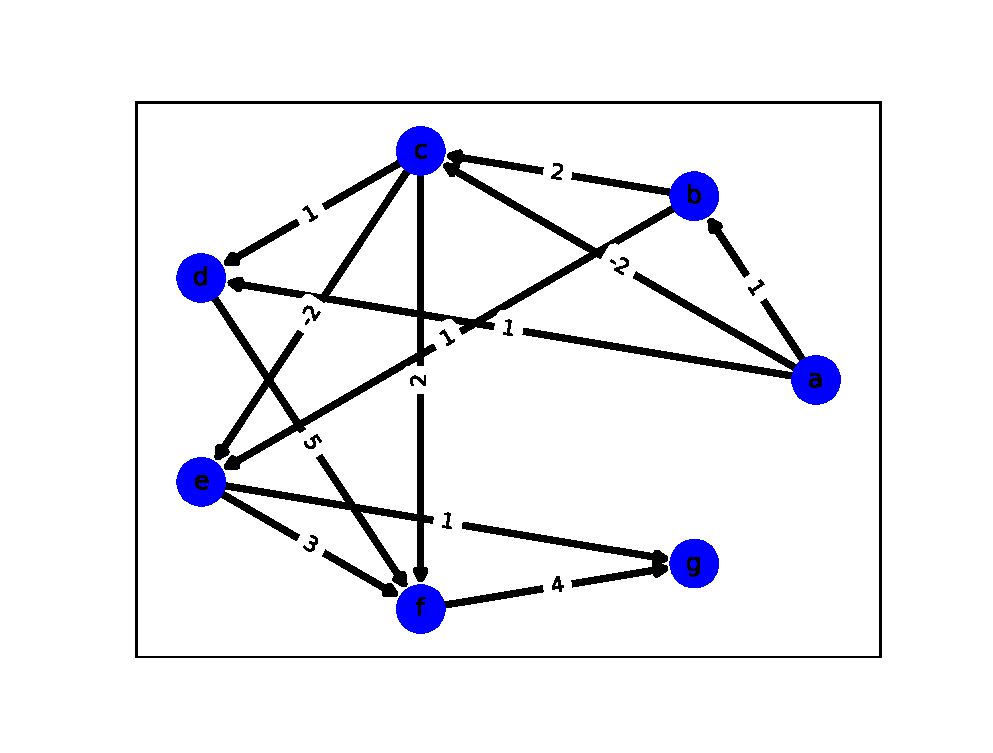
\includegraphics[scale = 0.5]{ejemplo6.eps}
    \label{figura6}
    \caption{7 nodos, inicio = a, final = g}
\end{figure}

En este ejemplo, al ejecutar el algoritmo \bell obtenemos la siguiente solución:
\begin{center}
    Distancia más corta:
    -3, ruta de la distancia más corta:
    ['a', 'c', 'e', 'g']
\end{center}

En el último ejemplo tenemos un grafo de igual manera dirigido con costos negativos:

\begin{figure}[h!t]
    \centering
    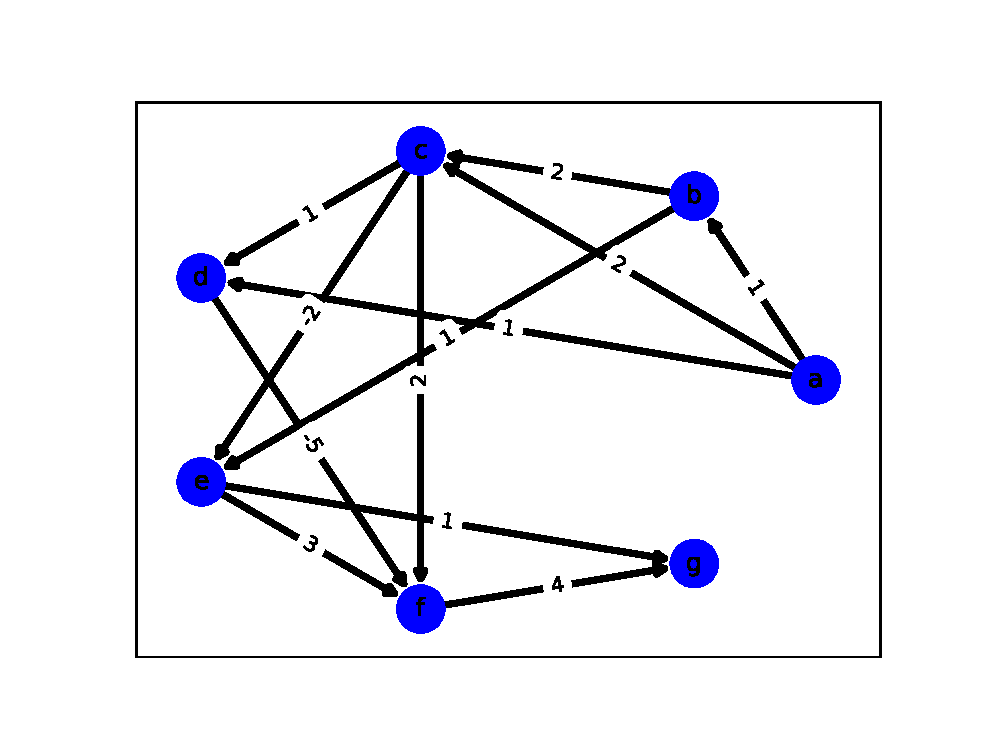
\includegraphics[scale = 0.5]{ejemplo7.eps}
    \label{figura7}
    \caption{7 nodos, inicio = a, final = g}
\end{figure}

Al ejecutar el código tenemos:
\begin{center}
    Distancia más corta:
    0, ruta de la distancia más corta:
    ['a', 'd', 'f', 'g']
\end{center}

\section{Repositorio}
Todo el código que se utilizo, notas y resultados lo podemos encontrar en \href{https://github.com/arnoldae9/redes.git}{git hub redes}, el cual es un repositorio personal.

\section{Networkx}
Como nota extra se utilizó la biblioteca \href{https://networkx.org/}{Networkx}.

En el archivo shortest\_path\_networkx que podemos encontrar en el mismo repositorio antes mencionado, podemos ver el código utilizado para generar las imágenes utilizadas en este reporte, asi como la implementación de unos ejemplos con el algoritmo de \dij y \bell porpios de la biblioteca Networkx respectivamente.
\section{Resultados}
Se utilizaron 3 grafos para el algoritmo de \dij de los cuales ninguno fallo, en el algoritmo de \bell se utilizaron 4 grafos (2 no dirigidos y 2 dirigidos) de los cuales tampoco falló ninguno.

Se utilizaron los siguientes libros:
\cite{chun2001core}
\cite{van1991guia}
\cite{van2017tutorial}, lo cuales se usaron de consulta para python.
\bibliography{biblio}
\bibliographystyle{alpha}



\end{document}

